% ==========================================================================================================================
\section{Arquitectura básica de SNMP}
% ==========================================================================================================================

\noindent
El modelo de administración de red que se utiliza para SNMP incluye los siguientes elementos:
\begin{itemize}
	\item Estación de gestión,
	\item Agente de Gestión,
	\item Base de información de gestión y
	\item Protocolo de Gestión de redes.
\end{itemize}

\noindent
En las secciones se enlistan las tareas para realizar la instalación y configuración de dichos elementos

% ==========================================================================================================================
\subsection{Instalación de la estación de gestión “Observium” en una máquina virtual}
% ==========================================================================================================================

\noindent
Para realizar la instalación de Observium sobre la máquina virtual debe tenerse previamente instalado un software de virtualización, para el caso utilizamos Virtual Box, así como la imagen ISO del sistema Observium a instalar. 

\noindent
\newline
\textbf{Paso 1:} Configuramos la red de la máquina virtual de Ubuntu, para eso debemos elegir el adaptador tipo puente, y dentro de las opciones avanzadas elegir el modo promiscuo. Como se ve a continuación: 

\pagebreak
\begin{figure}[htbp!]
	\centering
		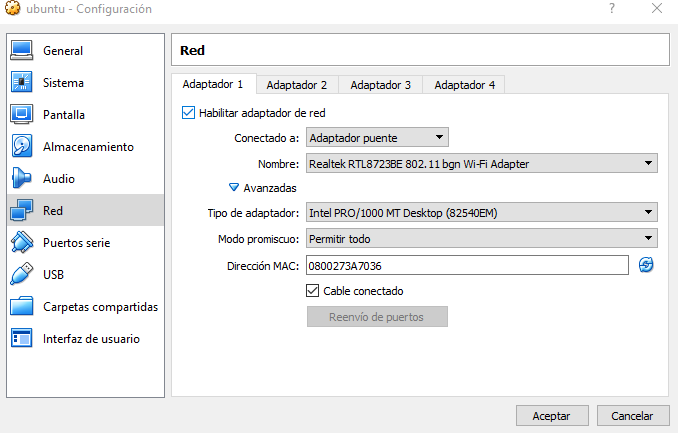
\includegraphics[width=0.8\textwidth]{images/desarrollo/instalarObservium_paso1.png}
	\caption{Instalación de observium: Paso 1.}
\end{figure}

\noindent
\textbf{Paso 2:} De las opciones de Virtual Box seleccionamos ''Almacenamiento'', luego ''Controlador IDE y seleccionamos la imagen ISO del sestema Observium. Como se muestra debajo: 

\begin{figure}[htbp!]
	\centering
		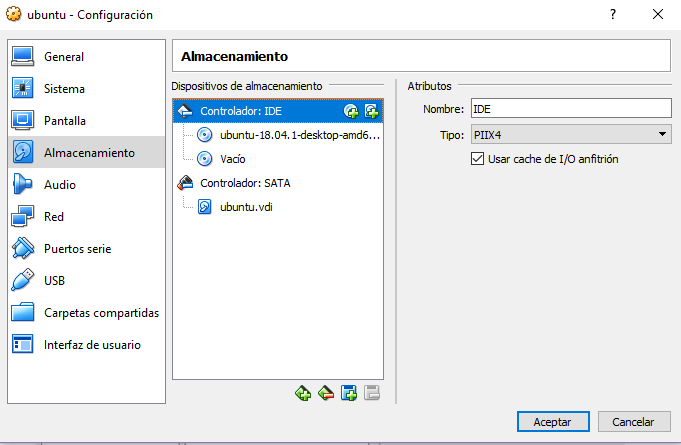
\includegraphics[width=0.8\textwidth]{images/desarrollo/instalarObservium_paso2.png}
	\caption{Instalación de observium: Paso 2.}
\end{figure} 

\pagebreak
\noindent
\textbf{Paso 3:} Creamos una nueva máquina virtual, e introducimos nombre, tipo y versión del sistema operativo a instalar. 

\begin{figure}[htbp!]
	\centering
		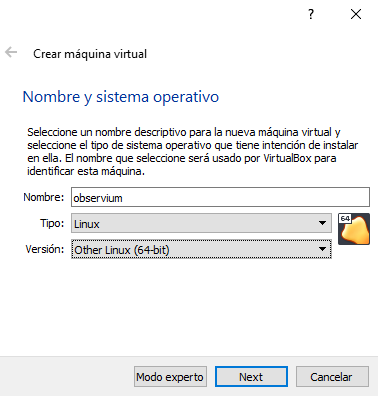
\includegraphics[width=0.5\textwidth]{images/desarrollo/instalarObservium_paso3.png}
	\caption{Instalación de observium: Paso 3.}
\end{figure} 

\noindent
\textbf{Paso 4:} Seleccionamos las características que tendrá nuestra máquina virtual para el sistema Observium. Tales como la memoria RAM o la capacidad de Disco duro. Como se muestra en las imágenes debajo. 

\begin{figure}[htbp!]
	\centering
		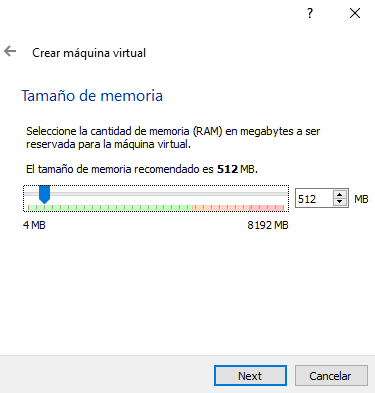
\includegraphics[width=0.5\textwidth]{images/desarrollo/instalarObservium_paso4a.png}
	\caption{Instalación de observium: Paso 4a.}
\end{figure} 

\pagebreak
\begin{figure}[htbp!]
	\centering
		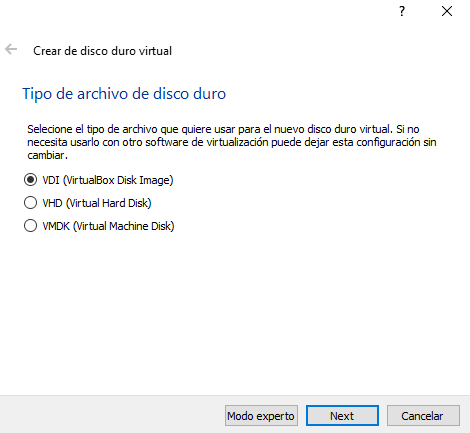
\includegraphics[width=0.5\textwidth]{images/desarrollo/instalarObservium_paso4b.png}
	\caption{Instalación de observium: Paso 4b.}
\end{figure} 

\noindent
\textbf{Paso 5:} Configuramos el adaptador de red, con las configuraciones que se observan en la imagen siguiente. 

\begin{figure}[htbp!]
	\centering
		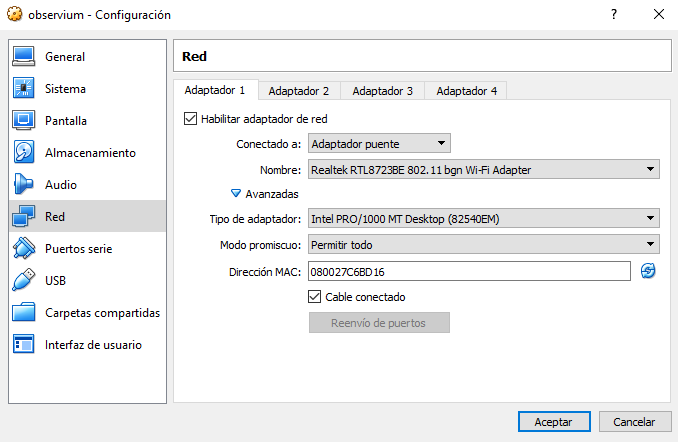
\includegraphics[width=0.8\textwidth]{images/desarrollo/instalarObservium_paso5.png}
	\caption{Instalación de observium: Paso 5.}
\end{figure} 

\pagebreak
\noindent
\textbf{Paso 6:} Se selecciona la imagen ISO con la cual va a correr el sistema.

\begin{figure}[htbp!]
	\centering
		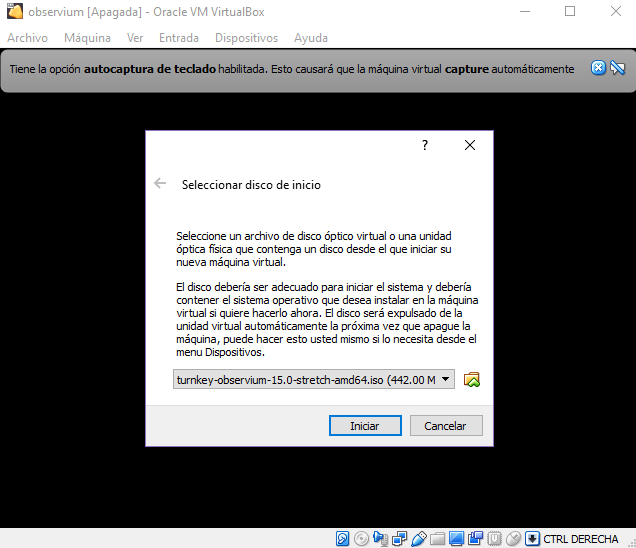
\includegraphics[width=0.6\textwidth]{images/desarrollo/instalarObservium_paso6.png}
	\caption{Instalación de observium: Paso 6.}
\end{figure}

\pagebreak
\noindent
\textbf{Paso 7:} Seleccionamos la opción de ''instalar'' mostrada en la siguiente pantalla. 

\begin{figure}[htbp!]
	\centering
		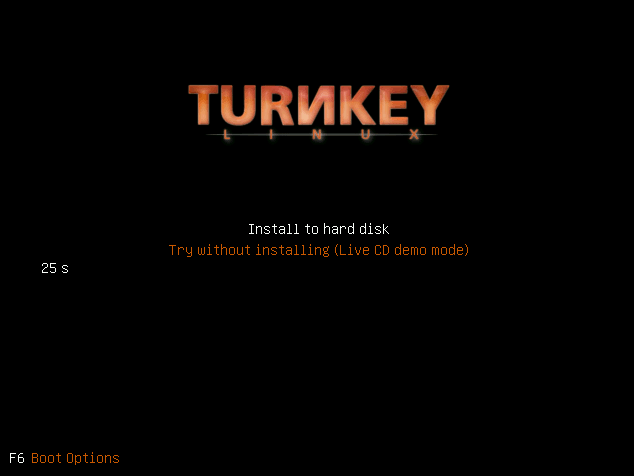
\includegraphics[width=0.8\textwidth]{images/desarrollo/instalarObservium_paso7.png}
	\caption{Instalación de observium: Paso 7.}
\end{figure}

\pagebreak
\noindent
\textbf{Paso 8:} De las pantallas a continuación siga el flujo, seleccionando las opciones marcadas. 

\begin{figure}[htbp!]
	\centering
		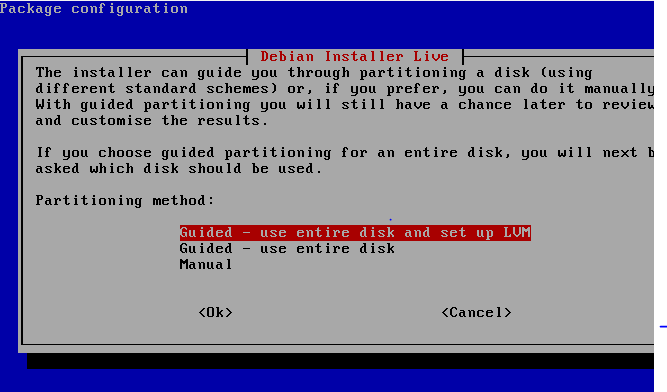
\includegraphics[width=0.8\textwidth]{images/desarrollo/instalarObservium_paso8.png}
	\caption{Instalación de observium: Paso 8.}
\end{figure}

\begin{figure}[htbp!]
	\centering
		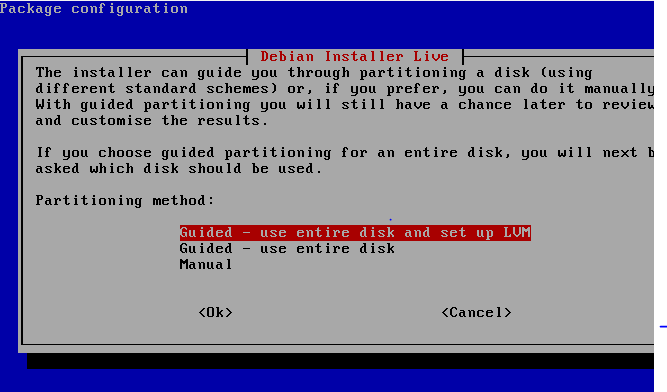
\includegraphics[width=0.8\textwidth]{images/desarrollo/instalarObservium_paso8.png}
	\caption{Instalación de observium: Paso 8.}
\end{figure}

\begin{figure}[htbp!]
	\centering
		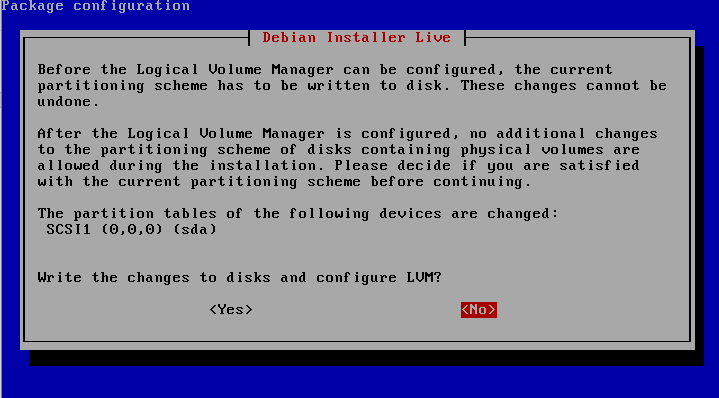
\includegraphics[width=0.8\textwidth]{images/desarrollo/instalarObservium_paso8b.png}
	\caption{Instalación de observium: Paso 8b.}
\end{figure}

\begin{figure}[htbp!]
	\centering
		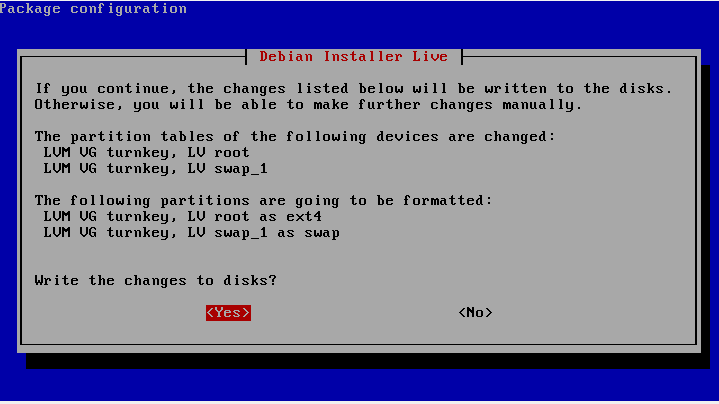
\includegraphics[width=0.8\textwidth]{images/desarrollo/instalarObservium_paso8c.png}
	\caption{Instalación de observium: Paso 8c.}
\end{figure}

\begin{figure}[htbp!]
	\centering
		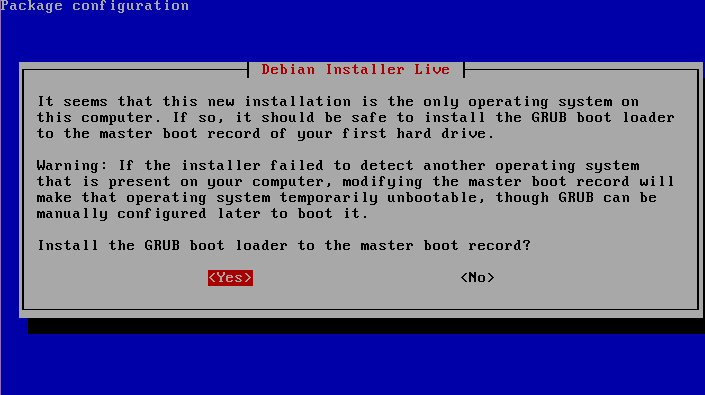
\includegraphics[width=0.8\textwidth]{images/desarrollo/instalarObservium_paso8d.png}
	\caption{Instalación de observium: Paso 8d.}
\end{figure}

\begin{figure}[htbp!]
	\centering
		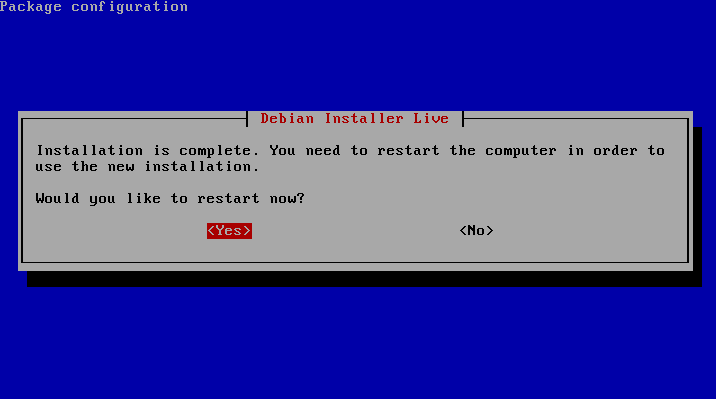
\includegraphics[width=0.8\textwidth]{images/desarrollo/instalarObservium_paso8e.png}
	\caption{Instalación de observium: Paso 8e.}
\end{figure}

\pagebreak
\noindent
\textbf{Paso 9:} Se establecen las contraseñas para la cuenta y la base de datos, así como un correo electrónico, como se observa en las imágenes debajo. 

\begin{figure}[htbp!]
	\centering
		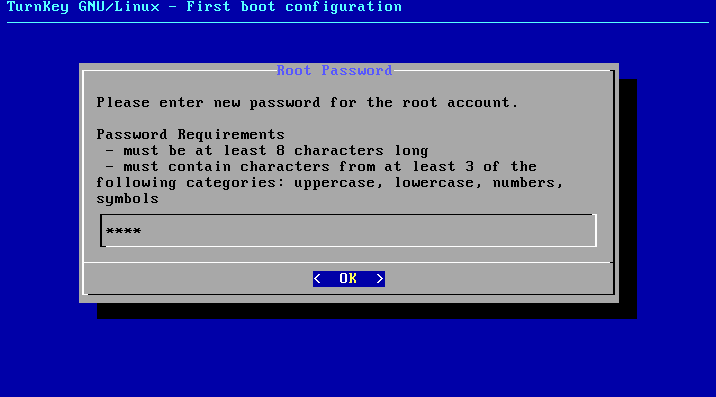
\includegraphics[width=0.8\textwidth]{images/desarrollo/instalarObservium_paso9a.png}
	\caption{Instalación de observium: Paso 9a.}
\end{figure}

\begin{figure}[htbp!]
	\centering
		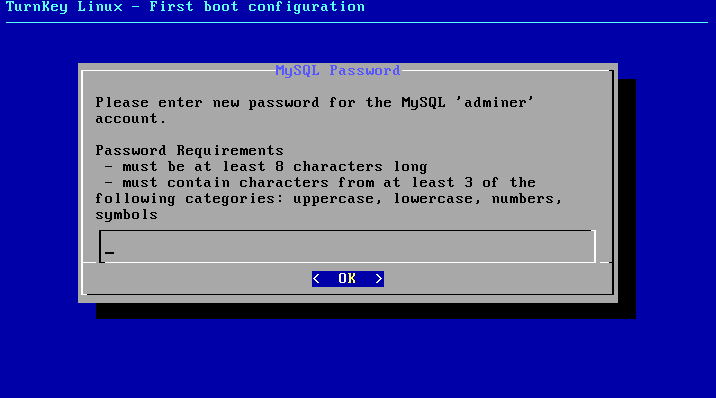
\includegraphics[width=0.8\textwidth]{images/desarrollo/instalarObservium_paso9b.png}
	\caption{Instalación de observium: Paso 9b.}
\end{figure}

\begin{figure}[htbp!]
	\centering
		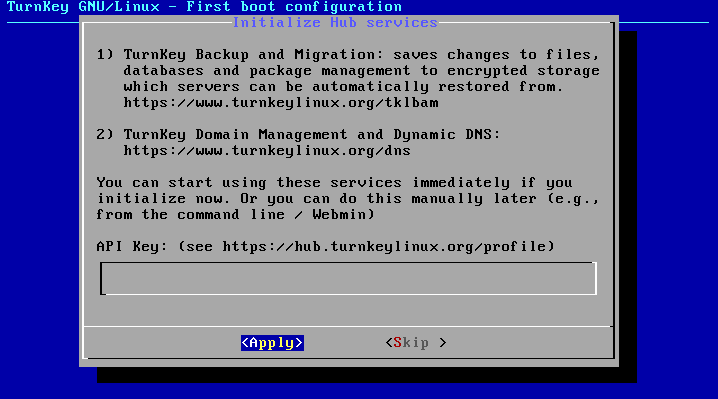
\includegraphics[width=0.8\textwidth]{images/desarrollo/instalarObservium_paso9c.png}
	\caption{Instalación de observium: Paso 9c.}
\end{figure}

\begin{figure}[htbp!]
	\centering
		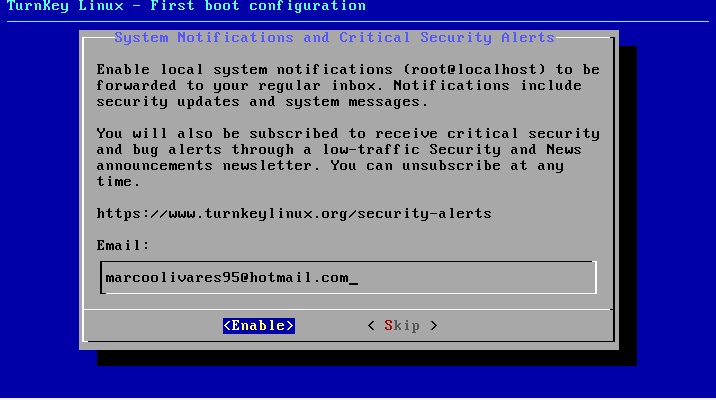
\includegraphics[width=0.8\textwidth]{images/desarrollo/instalarObservium_paso9d.png}
	\caption{Instalación de observium: Paso 9d.}
\end{figure}

\pagebreak
\noindent
\textbf{Paso 10:} Se selecciona la opción ''instalar'' y posteriormente ''reboot''. Como se muestra a continuación.

\begin{figure}[htbp!]
	\centering
		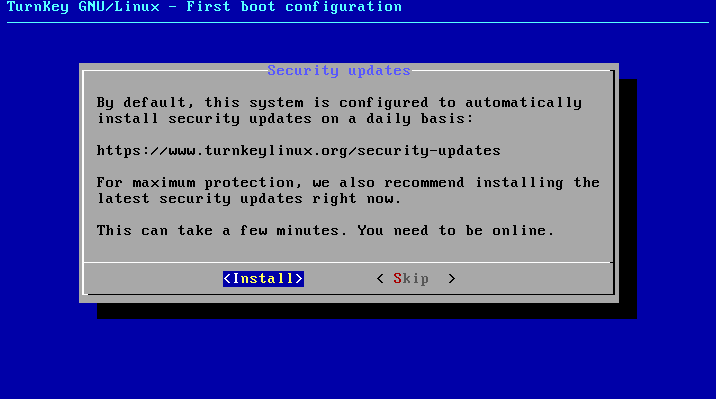
\includegraphics[width=0.8\textwidth]{images/desarrollo/instalarObservium_paso10a.png}
	\caption{Instalación de observium: Paso 10a.}
\end{figure}

\begin{figure}[htbp!]
	\centering
		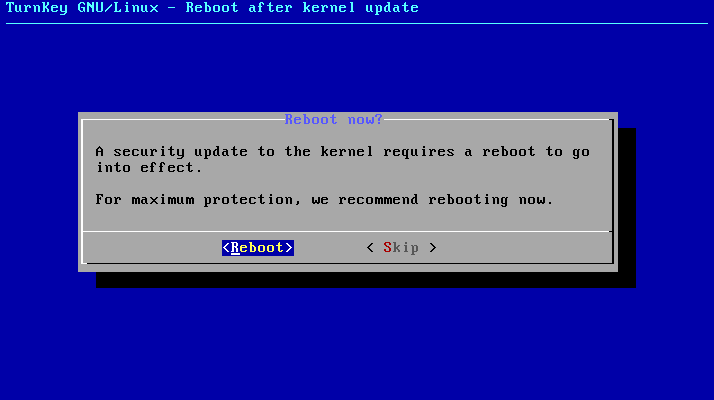
\includegraphics[width=0.8\textwidth]{images/desarrollo/instalarObservium_paso10b.png}
	\caption{Instalación de observium: Paso 10b.}
\end{figure}

% desde aquí empieza mi parte (Marco)

\pagebreak
\subsection{Publicar los agentes en Observium}
% ==========================================================================================================================

\noindent
\newline
\textbf{Paso 1:} Para dar de alta los agentes de Windows y Ubuntu, iniciaremos nuestro sistema operativo Observium, y en la terminar escribiremos el comando nano /etc/hosts.  En el archivo añadiremos las direcciones IP de nuestros agentes, seguidas de un espacio y el nombre del agente. Posteriormente se deben guardar los cambios pulsando ctrl + O. 

\begin{figure}[htbp!]
	\centering
		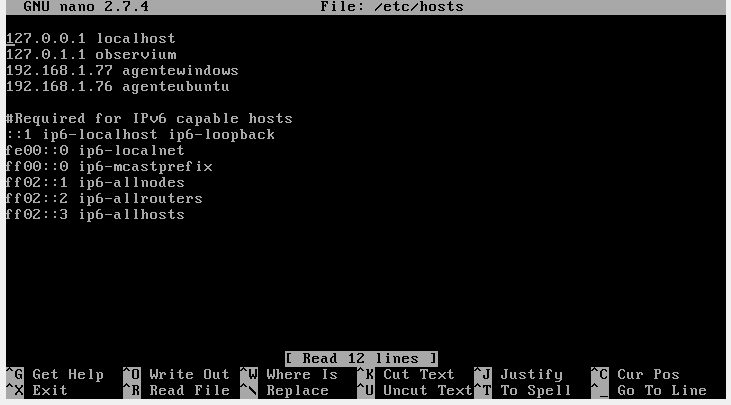
\includegraphics[width=0.8\textwidth]{images/desarrollo/agregar_agente1.png}
	\caption{Editando el archivo de hosts en Observium.}
\end{figure}

\noindent
\newline
\textbf{Paso 2:} Ya para concluir y comenzar el monitoreo de nuestros agentes, desde nuestro navegador web accederemos a la dirección IP de Observium, con la cual llegaremos a una página como la que se muestra a continuación.

\begin{figure}[htbp!]
	\centering
		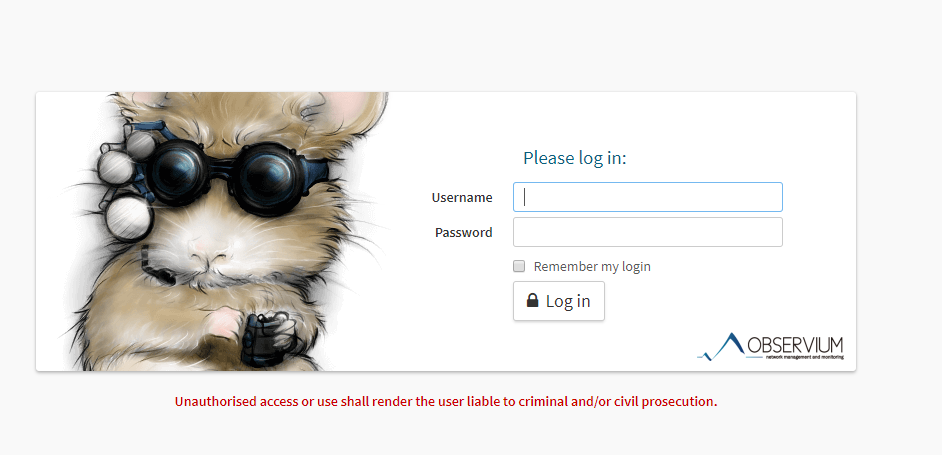
\includegraphics[width=0.8\textwidth]{images/desarrollo/agregar_agente2.png}
	\caption{Login de Observium.}
\end{figure}

\noindent
\newline
\textbf{Paso 3:}  El nombre de usuario a utilizar será siempre “admin”, y la contraseña será la que establecimos al momento de configurar nuestro sistema operativo Observium. Después de introducir nuestros datos, podremos visualizar la siguiente página.

\begin{figure}[htbp!]
	\centering
		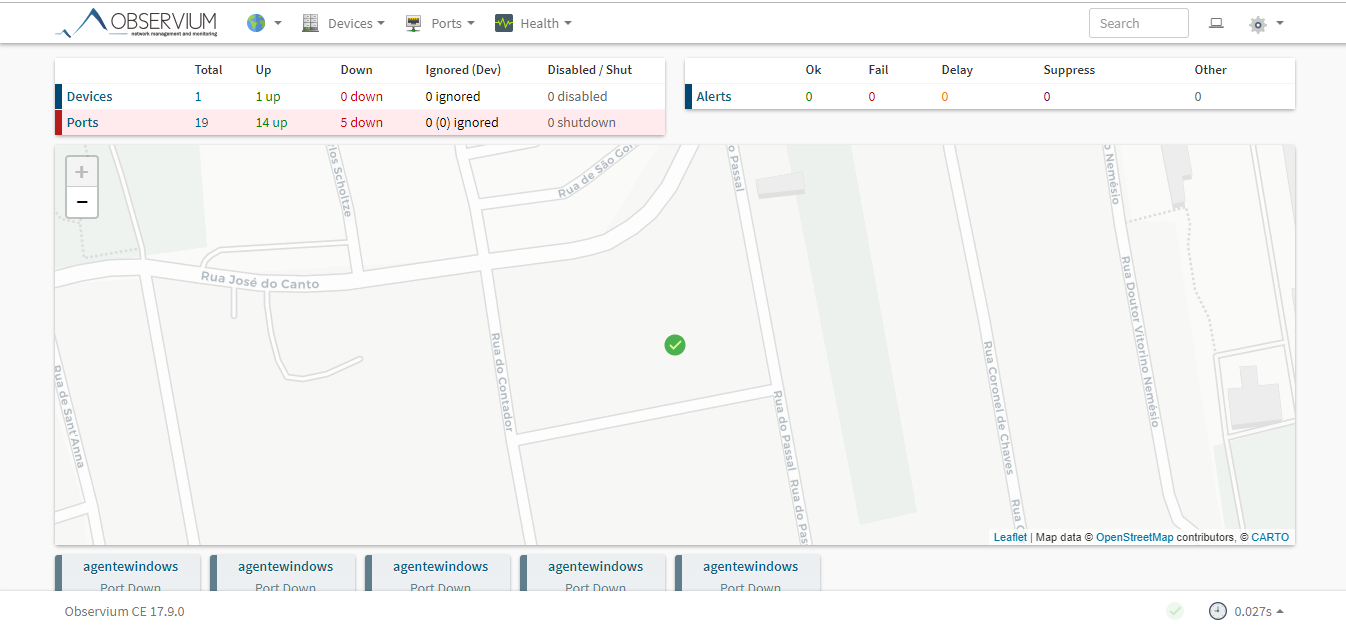
\includegraphics[width=0.8\textwidth]{images/desarrollo/agregar_agente3.png}
	\caption{Pantalla principal de Observium.}
\end{figure}

\noindent
\newline
\textbf{Paso 4:} Para monitorear nuestros agentes, iremos al menú devices, y seleccionaremos la opción add device. Posteriormente se nos solicitará introducir la información básica de nuestro agente, la cual es el nombre del host (asignado directamente en observium) y el nombre de la comunidad (asignado al momento de configurar el protocolo SNMP en el equipo). Es importante marcar la opción Skip PING, y después debemos dar clic en el botón Add device.

\begin{figure}[htbp!]
	\centering
		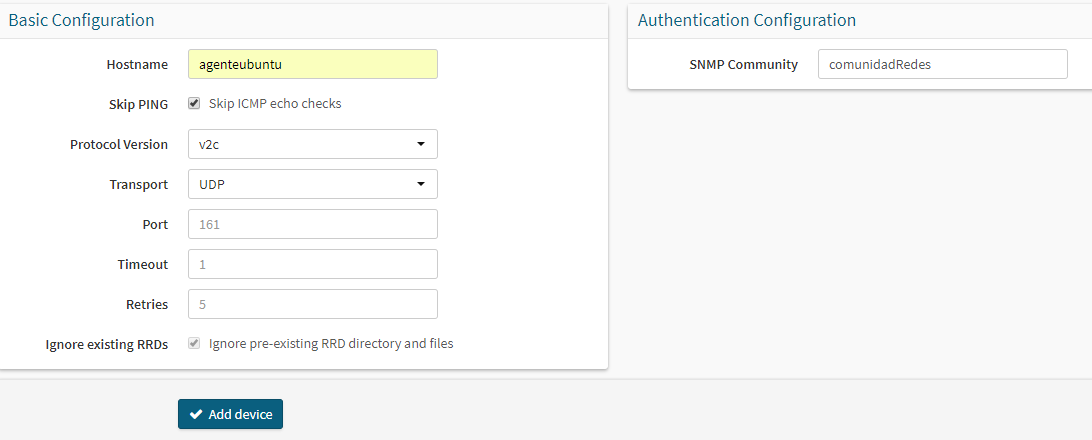
\includegraphics[width=0.8\textwidth]{images/desarrollo/agregar_agente4.png}
	\caption{Añadiendo agentes para monitorear.}
\end{figure}

\noindent
\newline
\textbf{Paso 5:} Si todos los pasos anteriores se realizaron correctamente, ahora nos será posible monitorear nuestro agente añadido con el paso anterior.

\begin{figure}[htbp!]
	\centering
		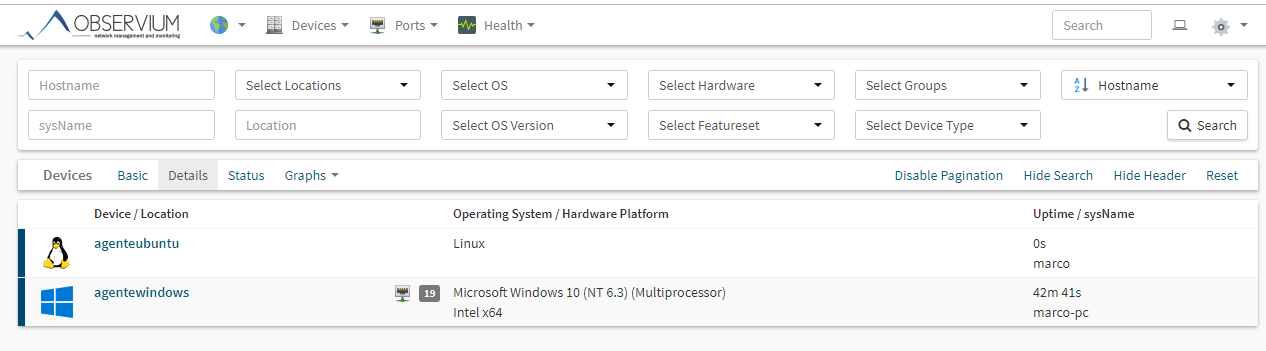
\includegraphics[width=0.8\textwidth]{images/desarrollo/agregar_agente5.png}
	\caption{Agentes agregados para su monitoreo.}
\end{figure}

\pagebreak
\subsection{Instalación y configuración de SNMP en Windows}
% ==========================================================================================================================
\noindent
\newline
\textbf{Paso 1:} Para configurar el protocolo SNMP en el sistema operativo Windows, primero es necesario activar el protocolo SNMP. Para ello, iremos al inicio, después al panel de control como se observa a continuación: 

\begin{figure}[htbp!]
	\centering
		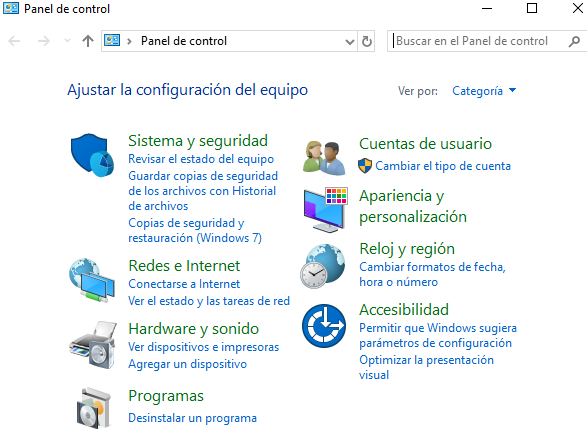
\includegraphics[width=0.8\textwidth]{images/desarrollo/configuracion_windows1.png}
	\caption{Vista general del panel de control.}
\end{figure}

\pagebreak
\noindent
\textbf{Paso 2:} En el panel de control, seleccionaremos el menú de programas. Posteriormente, en el apartado de programas y características seleccionaremos la opción de \textbf{activar o desactivar características de Windows.} 

\begin{figure}[htbp!]
	\centering
		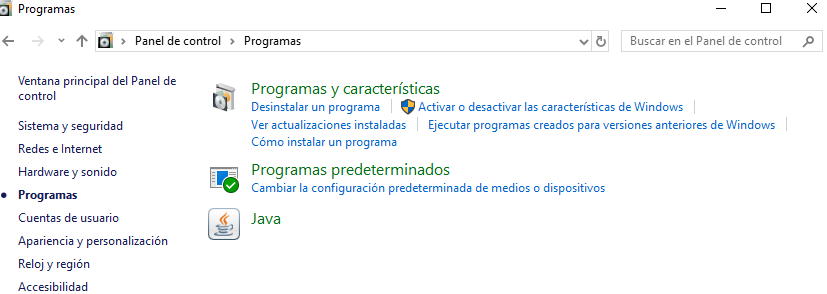
\includegraphics[width=0.8\textwidth]{images/desarrollo/configuracion_windows2.png}
	\caption{Opciones de programas y características en windows.}
\end{figure} 

\noindent
\textbf{Paso 3:} Observaremos una lista de las características de Windows, y entonces activaremos la opción \textbf{Protocolo Simple de Administración de Redes}, así como el \textbf{Proveedor WMI de SNMP.}

\begin{figure}[htbp!]
	\centering
		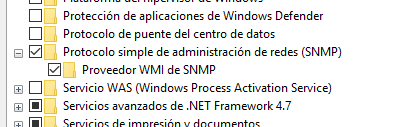
\includegraphics[width=0.5\textwidth]{images/desarrollo/configuracion_windows3.png}
	\caption{Activación del protocolo SNMP en Windows.}
\end{figure} 

\pagebreak
\noindent
\textbf{Paso 4:} Después, iremos a inicio, y a servicios. En la lista de servicios, buscaremos la opción de \textbf{Captura SNMP}, le daremos clic derecho, y después en la opción de iniciar. 

\begin{figure}[htbp!]
	\centering
		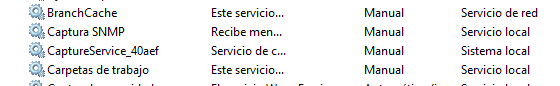
\includegraphics[width=0.5\textwidth]{images/desarrollo/configuracion_windows4.png}
	\caption{Servicio de captura SNMP en Windows}
\end{figure} 

\pagebreak
\noindent
\textbf{Paso 5:} Ahora buscaremos en la misma lista de servicios locales, el \textbf{servicio SNMP}, daremos clic derecho y seleccionaremos la opción de propiedades.
Iremos a la pestaña de \textbf{Capturas} y en el apartado del nombre de la comunidad, escribiremos el nombre de nuestra comunidad SNMP, y después daremos clic en el botón de agregar a la lista.


\begin{figure}[htbp!]
	\centering
		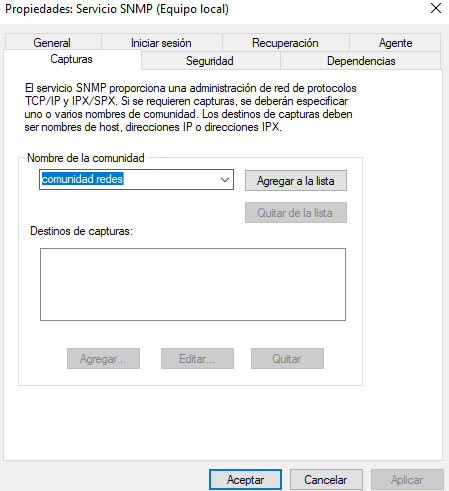
\includegraphics[width=0.5\textwidth]{images/desarrollo/configuracion_windows5.png}
	\caption{Añadiendo nuestra comunidad SNMP en Windows.}
\end{figure} 

\pagebreak
\noindent
\textbf{Paso 6:} Para terminar con la configuración del protocolo en Windows, iremos a la pestaña de captura. Le daremos permisos de lectura y escritura a nuestra comunidad SNMP, y seleccionaremos la opción que permite aceptar paquetes SNMP de cualquier host. Finalmente, daremos clic en el botón aceptar, e iniciaremos el servicio SNMP. 

\begin{figure}[htbp!]
	\centering
		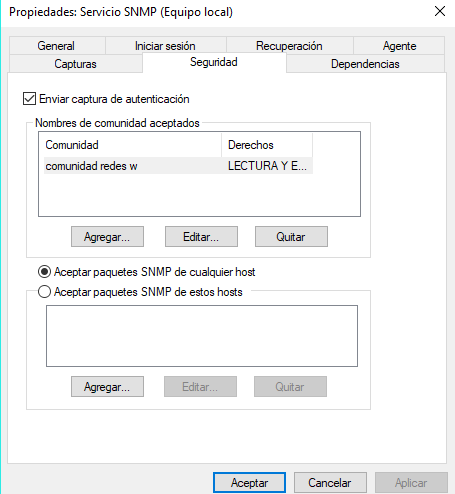
\includegraphics[width=0.8\textwidth]{images/desarrollo/configuracion_windows6.png}
	\caption{Configuración final del agente en Windows.}
\end{figure} 

\pagebreak
\subsection{Instalación y configuración de SNMP en Linux}
% ==========================================================================================================================

\noindent
\newline
\textbf{Paso 1:} Para el caso del agente de Linux, se utilizó una máquina virtual con ayuda de VirtualBox. Antes de proceder con la configuración del protocolo SNMP en el sistema operativo, primero se tiene que cambiar la configuración de red, seleccionando para ello el adaptador puente, y la opción \textbf{permitir todo} en el modo promiscuo. Dicha configuración se muestra a continuación.

\begin{figure}[htbp!]
	\centering
		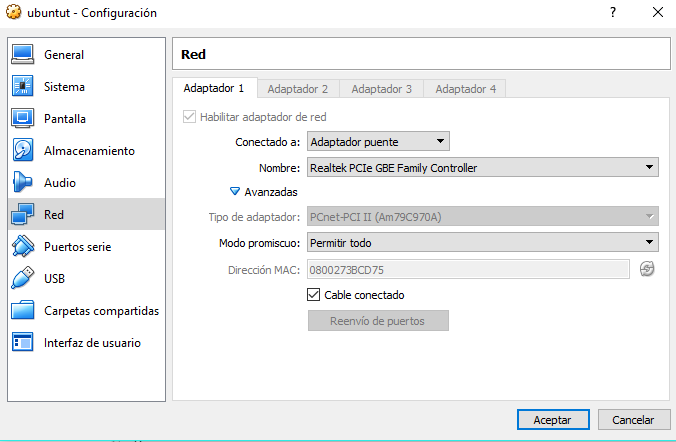
\includegraphics[width=0.8\textwidth]{images/desarrollo/configuracion_linux1.png}
	\caption{}
\end{figure}

\noindent
\newline
\textbf{Paso 2:} Una vez que se tiene esta configuración, se procede con la configuración del protocolo en Ubuntu. El primer paso en esta configuración es abrir una terminal y teclear el comando \textbf{sudo apt-get install snmp snmp} como se muestra a continuación.
También es necesario ejecutar el comando \textbf{sudo apt-get install snmp snmpd.}

\begin{figure}[htbp!]
	\centering
		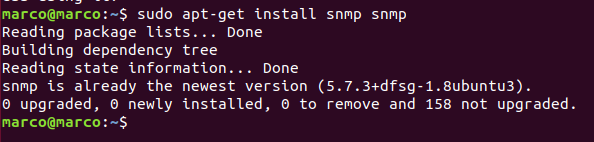
\includegraphics[width=0.8\textwidth]{images/desarrollo/configuracion_linux2.png}
	\caption{Ejecución de comandos para instalación de SNMP en Linux}
\end{figure}

\noindent
\newline
\textbf{Paso 3:}  Una vez realizados los pasos anteriores, ahora se comienza la configuración del agente. Para ello, se tecleará el comando \textbf{snmpconf -r none -g basic\_setup}. Primero se nos preguntará si deseamos configurar la información del grupo system de la MIB, y responderemos que sí (letra y).

\begin{figure}[htbp!]
	\centering
		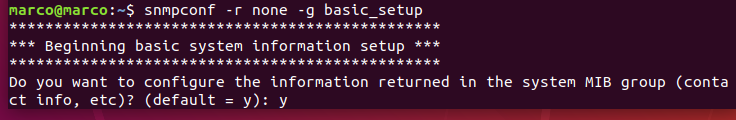
\includegraphics[width=0.8\textwidth]{images/desarrollo/configuracion_linux3.png}
	\caption{Inicio de la configuración del protocolo SNMP en Linux.}
\end{figure}

\noindent
\newline
\textbf{Paso 4:} Después se nos preguntará por la ubicación del sistema. En este caso podemos teclear lo que deseemos, haciendo referencia al lugar físico en donde se encuentra nuestro agente. 

\begin{figure}[htbp!]
	\centering
		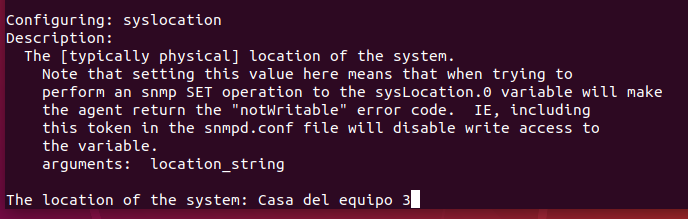
\includegraphics[width=0.8\textwidth]{images/desarrollo/configuracion_linux4.png}
	\caption{Estableciendo la ubicación del sistema.}
\end{figure}

\noindent
\newline
\textbf{Paso 5:} En la información de contacto debemos teclear toda la información deseada. Como ejemplo, teclearemos una dirección de correo electrónico.

\begin{figure}[htbp!]
	\centering
		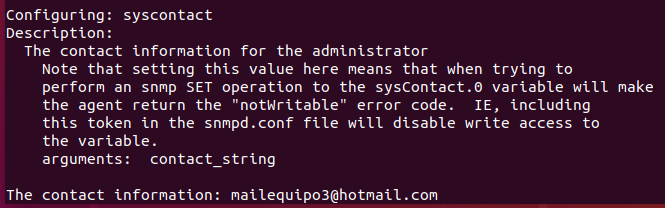
\includegraphics[width=0.8\textwidth]{images/desarrollo/configuracion_linux5.png}
	\caption{Estableciendo la información de contacto.}
\end{figure}

\pagebreak
\noindent
\newline
\textbf{Paso 6:} Para las siguientes preguntas, responderemos como se muestra en la siguiente imagen, y posteriormente se nos solicitará proporcionar el nombre de la comunidad.

\begin{figure}[htbp!]
	\centering
		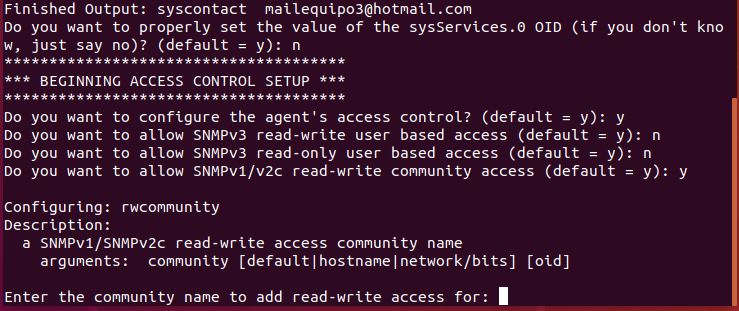
\includegraphics[width=0.8\textwidth]{images/desarrollo/configuracion_linux6.png}
	\caption{Opciones de configuración del protocolo SNMP y nombre de la comunidad.}
\end{figure}

\noindent
\newline
\textbf{Paso 7:} Tras escribir el nombre de nuestra comunidad, se nos preguntará si deseamos permitir el monitoreo de espacio en disco, procesos, entre otras cosas, y las respuestas dependerán de lo que deseamos monitorear. 

\begin{figure}[htbp!]
	\centering
		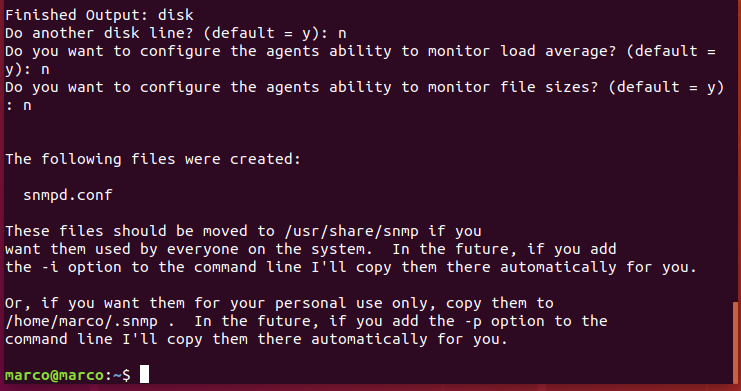
\includegraphics[width=0.8\textwidth]{images/desarrollo/configuracion_linux7.png}
	\caption{Configuración final del protocolo SNMP en Linux.}
\end{figure}

\pagebreak
\noindent
\newline
\textbf{Paso 8:} Finalmente, se nos generará un archivo llamado \textbf{snmpd.conf}, el cual deberemos mover al directorio \textbf{/etc/snmp/} usando el comando \textbf{sudo mv snmpd.conf /etc/snmp/snmpd.conf}.
Para verificar que el archivo se movió exitosamente, ahora teclearemos el comando \textbf{gedit /etc/snmp/snmpd.conf}, y se nos deberá mostrar un documento de texto como el que se muestra en las siguientes figuras.

\begin{figure}[htbp!]
	\centering
		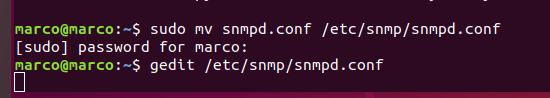
\includegraphics[width=0.8\textwidth]{images/desarrollo/configuracion_linux8.png}
	\caption{Comandos utilizados para mover de ubicación el archivo generado, así como para visualizarlo.}
\end{figure}

\begin{figure}[htbp!]
	\centering
		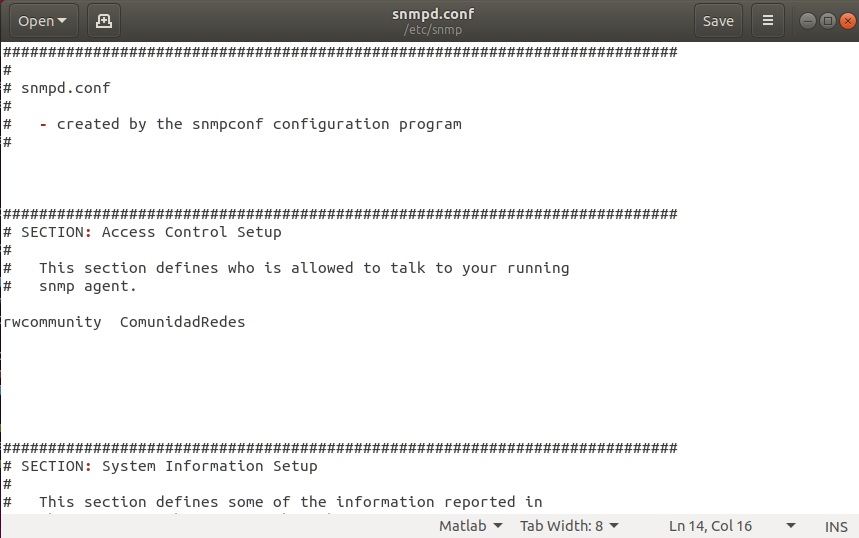
\includegraphics[width=0.8\textwidth]{images/desarrollo/configuracion_linux9.png}
	\caption{Contenido del archivo snmpd.conf.}
\end{figure}
